% ReAnimateAI --- Interim Report (~3 pages, single column = correct reading order)
% Overleaf: pdfLaTeX. PNGs: examples/grids/p01_grid.png ... p06 (or same folder as this file)

\documentclass[10pt,letterpaper]{article}

\usepackage[margin=0.85in]{geometry}
\usepackage{times}
\usepackage{graphicx}
\usepackage{booktabs}
\usepackage{hyperref}
\usepackage{caption}
\usepackage{microtype}

\newcommand{\etal}{et al.\ }
\captionsetup{font=small,skip=6pt}
\hypersetup{colorlinks=true,linkcolor=blue,citecolor=blue,urlcolor=blue}

\setlength{\parskip}{0.35ex}
\setlength{\textfloatsep}{10pt}

\title{ReAnimateAI: Intelligent Portrait Restoration Framework\\[0.3em]
\large Interim Report (Engineering Track)}

\author{
Keyurkumar Desai (MT25071) \and
Ishan Kumar (MT25069) \and
Rishabh Bajpai (MT25079) \and
Yash Kumar Saini (MT25054)
}
\date{}

\begin{document}
\maketitle

\begin{abstract}
\noindent
\textbf{Engineering Track.} \textbf{ReAnimateAI} targets portrait restoration: denoising, super-resolution, colorization, face enhancement, and optional subtle animation. We summarize problem scope, UI progress, related baselines and metrics, \emph{implemented} Zhang \etal colorization (Flask API + React/Vite web client), \textbf{measured CPU end-to-end latency}, qualitative failure modes, compute needs, team ownership, and next steps. Integration of the full multi-module pipeline remains in progress.
\end{abstract}

\section{(i) Problem Statement}
Historical and grayscale portraits often combine noise, blur, low resolution, fading, and missing color; manual restoration is slow and expert-dependent. \textbf{Input:} a single portrait (JPEG/PNG). \textbf{Target outputs:} restored, super-resolved, colorized, and face-enhanced imagery, plus optional short animation (e.g., blink, slight head motion). \textbf{Users:} families, archivists, and creators. \textbf{Interface:} browser upload, luminance preview, optional before/after comparison, and JPEG download. \textbf{Scope:} portrait-centric images; quality may degrade under extreme damage, heavy occlusion, or non-portrait scenes.

\section{(ii) User Interface \& Progress}
\textbf{Design.} A single-page \textbf{React + Vite} application calls a \textbf{Flask} REST endpoint (\texttt{/colorize}). The UI shows a luminance preview (color uploads are converted to grayscale automatically to match inference), runs colorization, provides a \textbf{Compare} slider and \textbf{download} of the result, and exposes quality presets (\texttt{fast} / \texttt{balanced} / \texttt{best}). Optional \textbf{Advanced} controls (CLAHE, saturation, sharpness) are collapsed by default.

\textbf{Implementation.} Backend: Python, Flask, OpenCV DNN, NumPy. Frontend: React~18, Vite~8. Dependencies are pinned via \texttt{requirements.txt} and the frontend lockfile. We used an AI-assisted editor (Cursor) for UI wiring and scripting.

\textbf{Status.} \emph{Implemented:} Zhang \etal Caffe colorization via OpenCV DNN, preprocessing/post-processing (including optional CLAHE and JPEG export), and latency-friendly API design. \emph{In progress:} restoration and SR modules, CodeFormer/GFP-style face enhancement, FOMM/old-photo animation, unified multi-stage orchestration, and a formal paired evaluation harness (PSNR/SSIM/LPIPS).

\section{(iii) Related Work \& Baselines}
\textbf{Colorization.} CNN methods predict chroma in Lab space; Zhang \etal~\cite{zhang2016colorful} uses class-rebalanced loss---we deploy public Caffe weights through OpenCV DNN. GAN-based colorization (DeOldify-style~\cite{deoldify_review}) can hallucinate plausible but incorrect colors under archival domain shift. \textbf{Face restoration.} CodeFormer~\cite{codeformer} and GFP-style priors recover detail but trade identity fidelity against texture synthesis. \textbf{Animation.} FOMM~\cite{fomm} and Wan \etal~\cite{oldphotos} enable motion transfer but risk flicker, warping, and identity drift. We plan swappable modules behind one API.

\section{(iv) Datasets \& Evaluation Metrics}
\textbf{Datasets (planned use):} ImageNet subset (controlled degradations), HumanFace8000 (portraits), VoxCeleb2 (motion), public historical scans (domain shift). \textbf{Image quality:} PSNR, SSIM, LPIPS where paired GT exists; optional small user study for color preference. \textbf{Faces / animation:} identity and landmark consistency; temporal consistency, frame stability, and cross-frame identity. \textbf{System:} end-to-end latency, RAM, optional GPU VRAM, per-module timing. \textbf{Hardware:} workstations with $\geq$16\,GB RAM; GPU for heavier models; Colab/Kaggle as needed.

\section{(v) Analysis of Results (Interim)}
We measured wall-clock time for six celebrity portraits using requests equivalent to the web UI (\texttt{grayscale\_only=1}, \texttt{balanced} preset). Mean latency is \textbf{2.29\,s} per image (min \textbf{1.29\,s}, max \textbf{4.16\,s}), indicating interactive use on CPU without a GPU server.

\vspace{0.5em}
\begin{center}
\captionof{table}{End-to-end \texttt{/colorize} latency (seconds).}
\label{tab:lat}
\small
\begin{tabular}{@{}lcccccc@{}}
\toprule
ID & p01 & p02 & p03 & p04 & p05 & p06 \\
\midrule
Time (s) & 4.16 & 2.35 & 1.65 & 1.29 & 1.63 & 2.64 \\
\midrule
\multicolumn{7}{@{}l}{\textbf{Mean:} 2.29\,s} \\
\bottomrule
\end{tabular}
\end{center}

\vspace{0.5em}
\noindent\textbf{Qualitative results.} Figure~\ref{fig:grids} shows Input$|$Output pairs for p01--p06 (thumbnails for page limit). \textbf{Failure modes:} \textbf{(A)} Ambiguity (p03): stripes and cluttered background map to similar luminance, so chroma is not unique. \textbf{(B)} High-frequency structure (p06): hair and fine detail can yield mild halos when coarse $ab$ is fused with high-resolution $L$. \textbf{(C)} Low resolution (p04, $366{\times}489$): few pixels under-specify facial geometry, producing slightly waxy colorization.

\begin{figure}[htbp]
\centering
\setlength{\tabcolsep}{2pt}
\begin{tabular}{@{}ccc@{}}
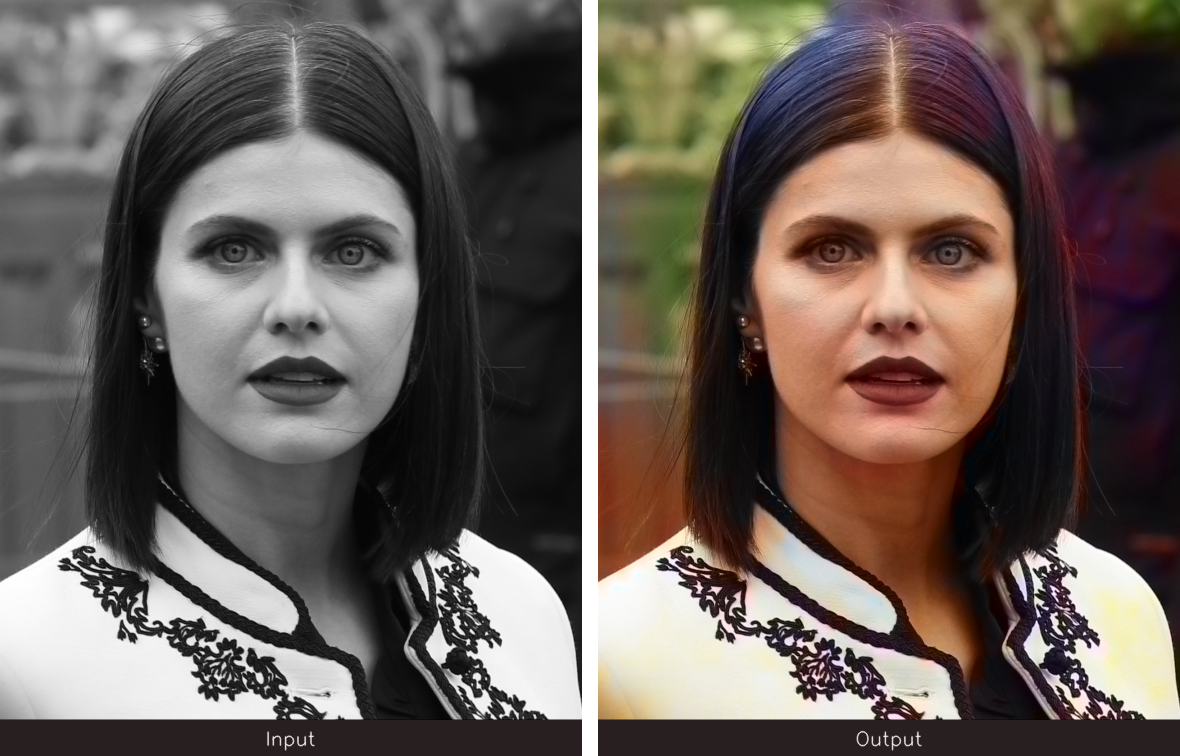
\includegraphics[width=0.31\linewidth,height=1.05in,keepaspectratio]{examples/grids/p01_grid.png} &
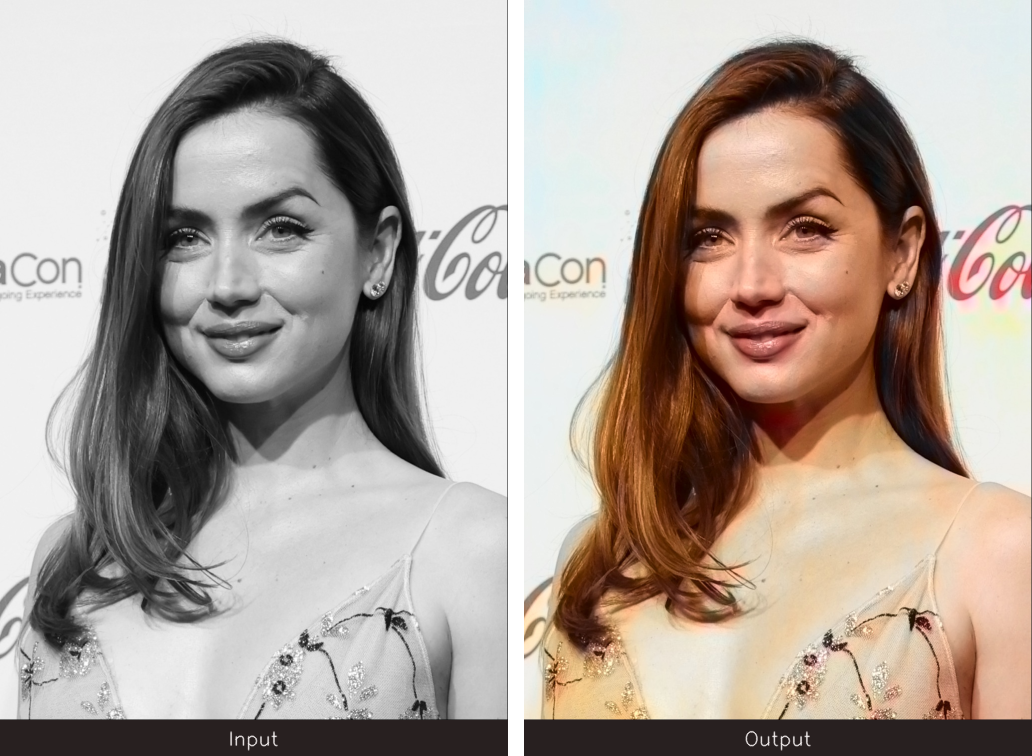
\includegraphics[width=0.31\linewidth,height=1.05in,keepaspectratio]{examples/grids/p02_grid.png} &
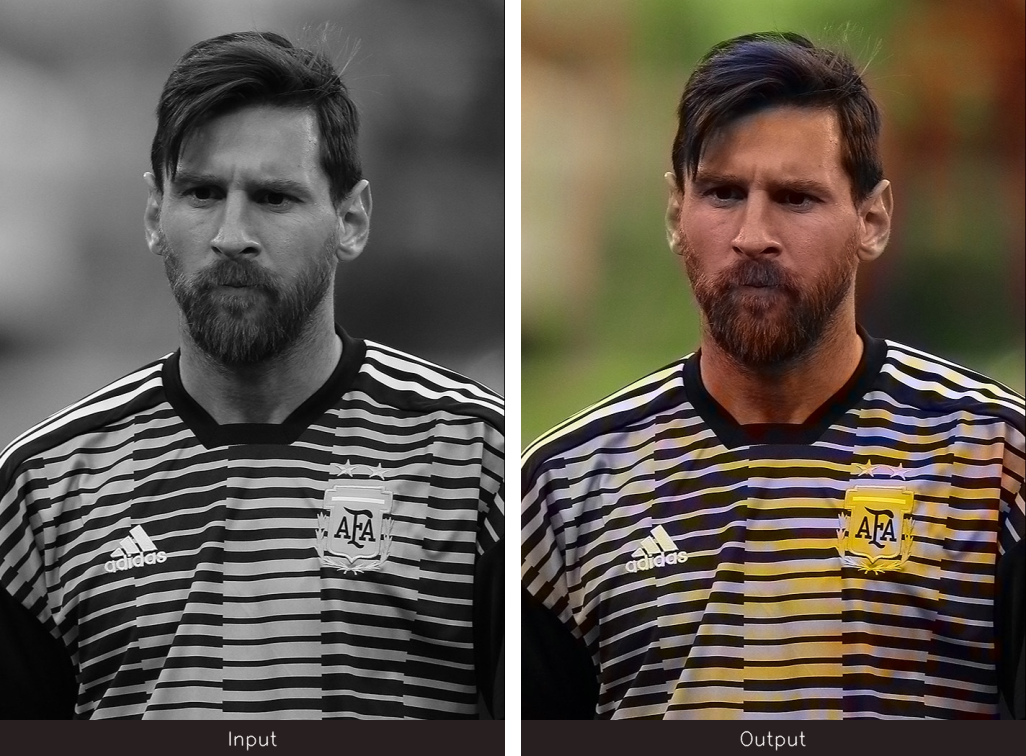
\includegraphics[width=0.31\linewidth,height=1.05in,keepaspectratio]{examples/grids/p03_grid.png} \\[2pt]
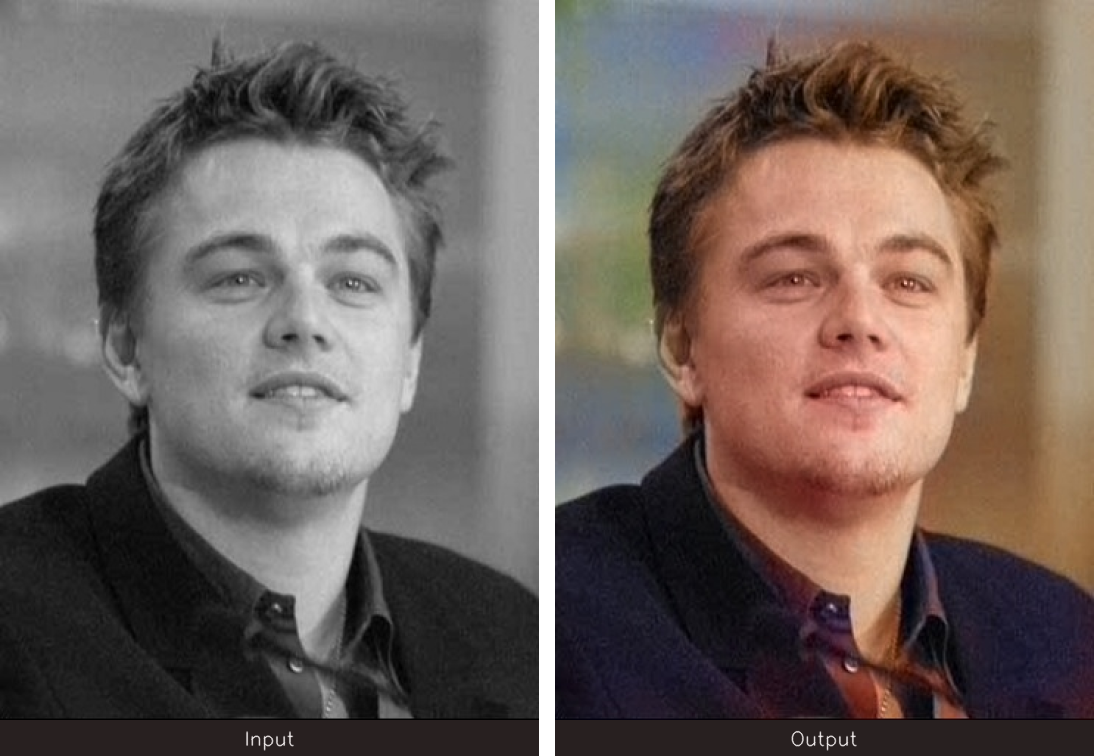
\includegraphics[width=0.31\linewidth,height=1.05in,keepaspectratio]{examples/grids/p04_grid.png} &
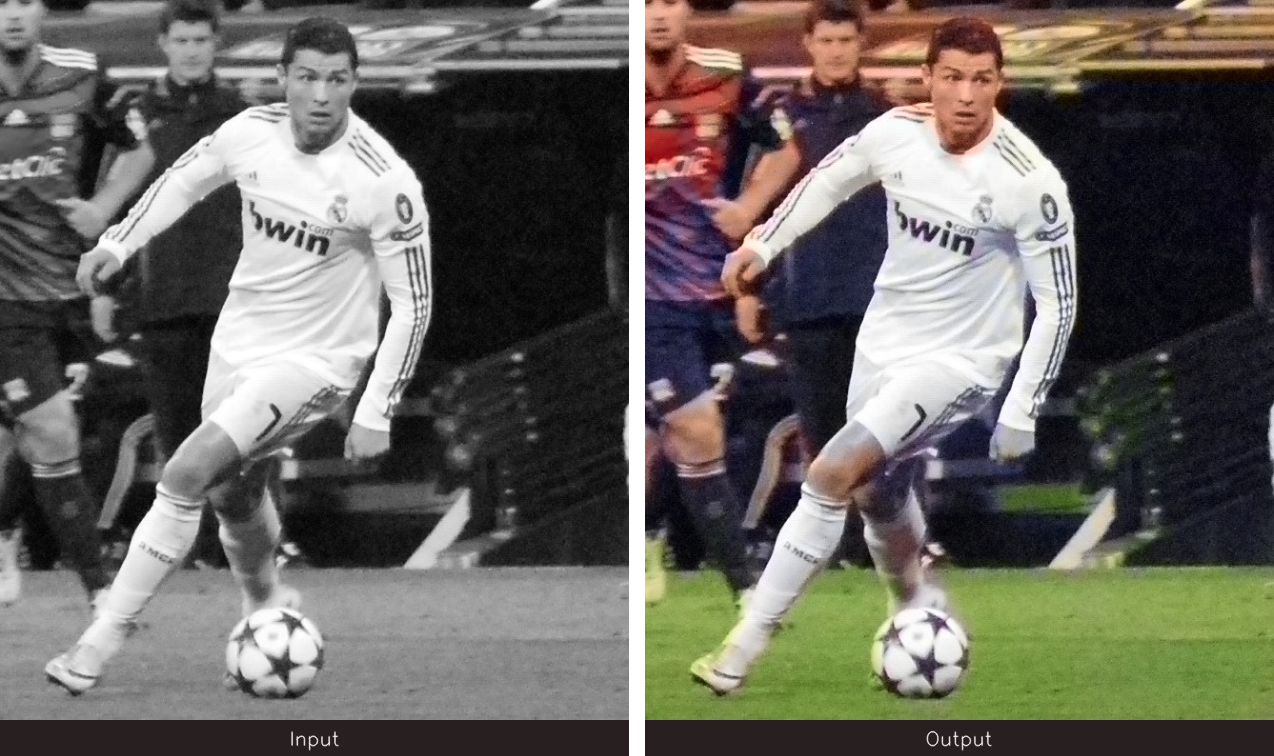
\includegraphics[width=0.31\linewidth,height=1.05in,keepaspectratio]{examples/grids/p05_grid.png} &
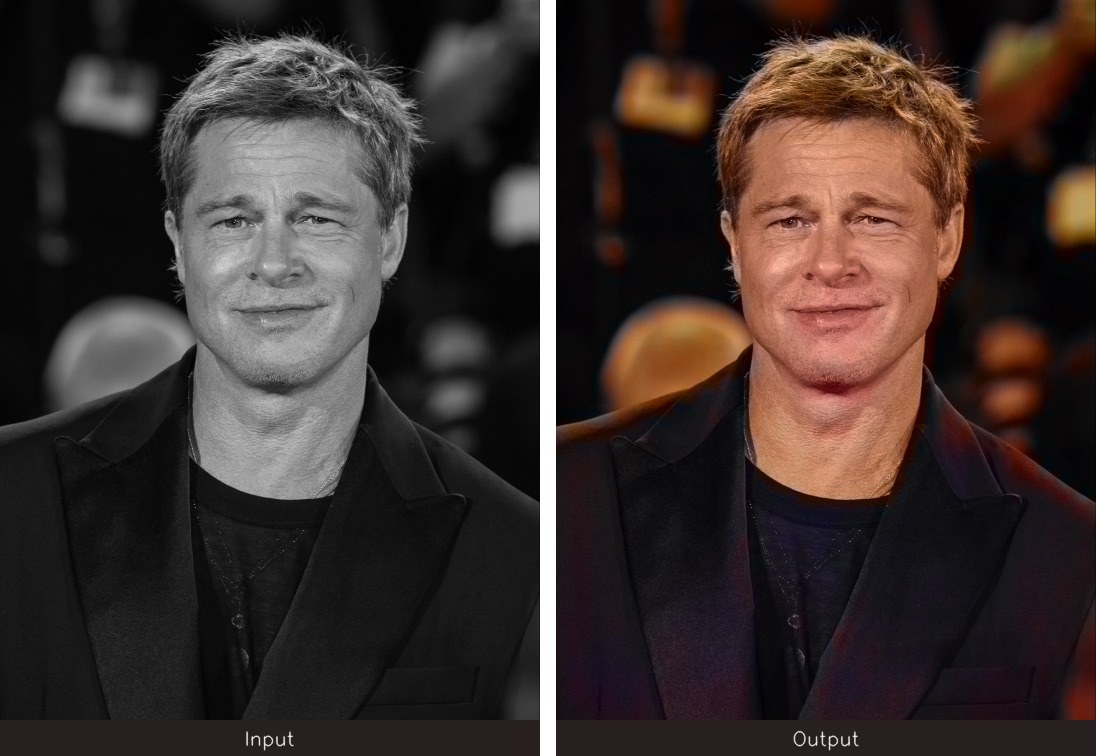
\includegraphics[width=0.31\linewidth,height=1.05in,keepaspectratio]{examples/grids/p06_grid.png} \\
\end{tabular}
\caption{Input$|$Output thumbnails (p01--p06). See \S(v) for failure discussion (p03, p04, p06).}
\label{fig:grids}
\end{figure}

\section{(vi) Compute Requirements}
The colorization path runs on \textbf{CPU} (OpenCV DNN) with model assets $\approx$\,130\,MB. Table~\ref{tab:lat} reflects observed interactive performance. Upcoming SR, face GANs, and animation are expected to require \textbf{GPU} memory and longer inference; we will report VRAM and throughput when integrated.

\section{(vii) Individual Tasks}
\begin{center}
\small
\begin{tabular}{@{}p{0.22\linewidth}p{0.28\linewidth}p{0.44\linewidth}@{}}
\toprule
\textbf{Member} & \textbf{Ownership} & \textbf{Interim focus} \\
\midrule
Keyurkumar Desai & Restoration + evaluation & Synthetic degradations; paired metrics; failure taxonomy. \\
Ishan Kumar & Super-resolution & SR baseline integration; latency and VRAM profiling. \\
Rishabh Bajpai & Colorization + UI & OpenCV DNN integration; React/Vite UI; deployment path. \\
Yash Kumar Saini & Animation & FOMM / old-photo animation; temporal stability metrics. \\
\bottomrule
\end{tabular}
\end{center}

\section{(viii) Next Steps}
Orchestrate remaining modules under one API with clear I/O contracts; add input validation, file-size limits, and structured errors; run quantitative colorization benchmarks on a fixed split; integrate SR, face restoration, and animation with per-module timing; conduct a small perceptual study once the full pipeline is stable.

\begin{thebibliography}{99}
\bibitem{zhang2016colorful}
R.~Zhang, P.~Isola, and A.~A. Efros.
\newblock Colorful image colorization.
\newblock In \emph{ECCV}, 2016.

\bibitem{deoldify_review}
DeOldify: review and implementation of automatic colorization (see e.g.\ arXiv:2101.04061 / IPOL-style surveys).

\bibitem{codeformer}
S.~Zhou \etal
\newblock Towards robust blind face restoration with codebook lookup transformer.
\newblock In \emph{NeurIPS}, 2022.

\bibitem{fomm}
A.~Siarohin \etal
\newblock First order motion model for image animation.
\newblock arXiv:2003.00196, 2019.

\bibitem{oldphotos}
Z.~Wan \etal
\newblock Bringing old photos back to life.
\newblock In \emph{CVPR}, 2020.
\end{thebibliography}

\end{document}
